\section{Wprowadzenie}
Badanie elektrokardiograficzne, dzięki swej dostępności i łatwości wykonania stanowi jedną z najczęściej wykorzystywanych metod rozpoznawania zaburzeń w pracy serca. Uzyskiwany przy jego pomocy sygnał EKG dostarcza informacji o elektrycznej aktywności mięśnia sercowego jako różnicę potencjałów pomiędzy dwoma elektrodami.

Jednym z najbardziej charakterystycznych elementów typowego sygnału EKG są zespoły QRS. Jest to układ trzech załamków opisujących proces depolaryzacji mięśnia. Ideowy schemat EKG, wraz z kompleksem QRS przedstawiono na rysunku \ref{fig:qrs-complex}.


\begin{figure}[H]
	\centering
	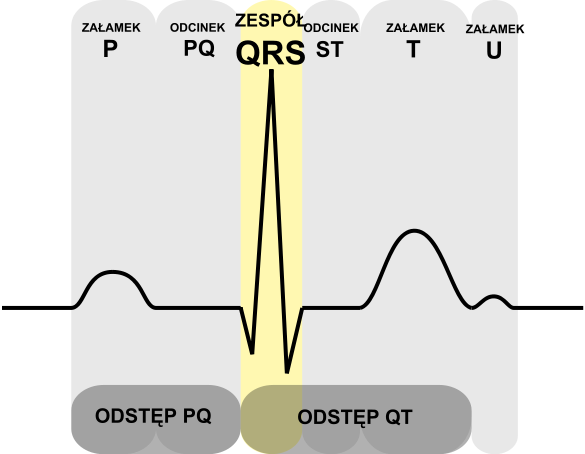
\includegraphics[width=12cm]{img/qrs-complex}
	\caption{Ideowy schemat sygnału EKG. Źródło: \cite{qrs-wiki}}
	\label{fig:qrs-complex}
\end{figure}

Na podstawie charakteru zespołu QRS diagnozować można szereg dysfunkcji serca. Wykorzystanie w tym celu zautomatyzowanych procedur diagnostycznych pozwala na zwiększenie prawdopodobieństwa wykrycia nieprawidłowości i przyśpiesza proces badania. Wymaga to jednak wyodrębnienia grup kompleksów o podobnych parametrach. Uzyskane grupy powinny odwzorowywać najczęściej występujące zaburzenia pracy serca.

\section{Koncepcja proponowanego rozwiązania}

Autorzy badali możliwość wykorzystania algorytmu kNN (\textit{k Nearest Neighbours}) oraz jego rozszerzonej wersji, eNN (\textit{extended Nearest Neighbours}) do zaprojektowania zautomatyzowanego procesu klasyfikacji zespołów QRS do predefiniowanych grup. Opis algorytmów przedstawiono w rozdziałach \ref{chap:knn} i \ref{chap:enn}.

Metody klasy \textit{NN} wymagają przedstawienia danych wejściowych w postaci wektora cech o ustalonym wymiarze. Zdecydowano się wykorzystać w tym celu dane dostępne w opracowaniu \cite{heart-class-module}. Zmodyfikowano klasyfikację grup w taki sposób, aby odwzorowywała wszystkie klasy definiowane w dokumentacji bazy \textit{MIT-BIH} \cite{mitdb}.

Dane wejściowe opisywane są wektorem składającym się z osiemnastu cech. Wektor zawiera informacje na temat chwil wystąpienia kolejnych elementów kompleksu QRS a także wartości sygnału w istotnych chwilach. Jedna z kolumn - chwila wystąpienia załamka R - związana jest jednoznacznie z badanym sygnałem EKG i nie pozwala na klasyfikację w uogólnionym zbiorze danych, z tego powodu jest ignorowana w zaprojektowanym rozwiązaniu.

Celem projektu było zaprojektowanie prototypu proponowanego rozwiązania przy użyciu oprogramowania \textit{Matlab}, a także zgodnej z nim implementacji w języku \textit{C++}. Wykorzystano również bibliotekę \textit{Eigen} \cite{eigen-www}, pozwalającą na optymalizację operacji matematycznych na macierzach i wektorach.

Cykl działania aplikacji podzielić można na dwa etapy.
\begin{enumerate}
	\item Proces uczenia.
	
	Program uczony jest przy użyciu wybranego zbioru danych wejściowych wraz z poprawną klasyfikacją każdego wektora. Dane te są zapamiętywane i wykorzystywane na kolejnym etapie pracy.
	
	\item
	Klasyfikacja danych wejściowych.
	
	Aplikacja pozwala na klasyfikację dowolnej liczby wektorów danych, porównując je z posiadanym zbiorem referencyjnym. Wyjściem programu na wejście zawierające jeden wektor testowy jest klasa, do której został on przypisany.
\end{enumerate}

Test poprawności działania implementacji wymagał podzielenia znanego zbioru danych na podzbiory - uczący i testowy, wraz ze związanymi z nimi klasami. Przyjęto podział w stosunku siedem do trzech. Działanie algorytmu badane było niezależnie dla każdego pliku wejściowego.

\section{Dane wejściowe}
Na etapie testowania działania proponowanych algorytmów wykorzystano dane zgromadzone w ramach biblioteki arytmii pracy serca \textit{MIT-BIH}. Zbiór zawiera czterdzieści osiem zapisów trzydziestominutowych badań \textit{EKG}. Dwadzieścia trzy nagrania stanowią losowo wybrany podzbiór bazy zawierającej zapis kilku tysięcy badań, natomiast pozostałe dwadzieścia pięć nagrań to zbiór dobrany w taki sposób, by zawierał istotne lecz rzadziej występujące klasy arytmii. Dane zawarte w bazie zawierają również precyzyjną klasyfikację kompleksów \textit{QRS} dla każdego nagrania.

Dane zawarte w bazie danych nie mogą być bezpośrednio wykorzystane do przeprowadzenia procesu klasyfikacji. Sygnał wejściowy musi zostać poddany filtracji oraz ograniczony do wektorów cech opisujących kolejne zespoły \textit{QRS}. W ramach projektu wykorzystano wstępnie przygotowane dane wejściowe, zawierające wektory cech i adnotacje klas.

Wykorzystując opisany zbiór wejściowy, badano skuteczność detekcji klas przez algorytm. Sprawdzano również możliwość zaprojektowania zbioru uczącego w taki sposób, aby jak najlepiej reprezentował on klasy sygnału, maksymalizując skuteczność detekcji w zbiorze zawierającym wszystkie pliki danych.